%%%%%%%%%%%%%%%%%%%%%%%%%%%%%%%%%%%%%%%%%%%%%%%%%%%%%%%%%%%%%%%%%%%%%%
% How to use writeLaTeX: 
%
% You edit the source code here on the left, and the preview on the
% right shows you the result within a few seconds.
%
% Bookmark this page and share the URL with your co-authors. They can
% edit at the same time!
%
% You can upload figures, bibliographies, custom classes and
% styles using the files menu.
%
%%%%%%%%%%%%%%%%%%%%%%%%%%%%%%%%%%%%%%%%%%%%%%%%%%%%%%%%%%%%%%%%%%%%%%

\documentclass[12pt]{article}

\usepackage{sbc-template}

\usepackage{amsmath}

\usepackage{graphicx,url}

%\usepackage[brazil]{babel}   
\usepackage[utf8]{inputenc}  

     
\sloppy

\title{Relatório da Avaliação RA3}

\author{Vinicius de Andrade Deolindo\inst{1}, Gustavo Silveira e Silva\inst{1}}

\address{Pontifícia Universidade Católica do Paraná (PUCPR) }

\begin{document} 

\maketitle

\begin{abstract}
This report explores the implementation and performance analysis of a custom HashMap data structure, 
using different hashing functions and bucket sizes.
Three different hashing methods were evaluated — modulo, multiplicative and fractional multiplicative — 
across various dataset and bucket size configurations to understand their efficiency in insert and fetch operations.
Metrics collected while running the experiments were plotted on graphs to examine performance trends,
facilitating a comparative analysis of execution time between functions and configurations.
\end{abstract}

\begin{resumo}
Este relatório explora a implementação e análise de desempenho de uma estrutura de dados HashMap personalizada, 
utilizando diferentes funções de hashing e tamanhos de buckets.
Foram avaliados três métodos de hashing distintos — modulo, multiplicativo e multiplicativo fracionário — 
em várias configurações de tamanho de conjuntos de dados e buckets para entender sua eficiência em operações de inserção e busca.
As métricas coletadas durante a execução dos experimentos foram plotadas em gráficos para examinar as tendências de desempenho,
facilitando uma análise comparativa do tempo de execução entre as funções e configurações. 
\end{resumo}

\section{Introdução}
Hash tables (ou tabelas de dispersão) são estruturas onde o tempo de busca e inserção idealmente ocorre em tempo constante, $O(1)$. 
As estruturas são baseadas no conceito de \textit{hashing}, onde uma função transforma uma chave arbitrária em um índice que determina a localização na tabela do valor associado.
No entanto, funções imperfeitas de hashing geram colisões, onde várias chaves resultam na mesma índice, 
e a implementação tem que estar equipada para lidar com essas colisões. Neste projeto, lidamos com colisões com "encadeamento", onde cada elemento da tabela é, na verdade,
uma lista encadeada em que cada nó contém a chave original da inserção, que é comparada na busca.

Foram testadas três funções de hash diferentes: 
$$\text{Mod} = \text{hash}(k, m) = k \bmod m$$
$$\text{Multiplicativo} = \text{hash}(k, m) = \left| (A \cdot k) \bmod m \right|$$
$$\text{Multiplicativo fracional} = \text{hash}(k, m) = \left\lfloor m \cdot ((A \cdot k) \bmod 1) \right\rfloor$$
Cada função apresenta características distintas, com impacto direto na distribuição das chaves na tabela e, consequentemente, no desempenho da estrutura.
Para a análise de desempenho, foram amostrados o tempo de inserção e busca de elementos.

As estruturas foram populadas com 1 milhão, 5 milhões e 20 milhões de registros gerados aleatoriamente, 
onde cada registro é composto por um código (usado como chave), que é um inteiro aleatório de 9 digitos, e um valor (usado como valor), que é um inteiro aleatório.
Cada conjunto de registros foi testado com tabelas de 100 mil, 500 mil e 1 milhão de elementos.

\section{Inserção de registros}

\subsection{Amostras}

\begin{figure}[ht]
\centering
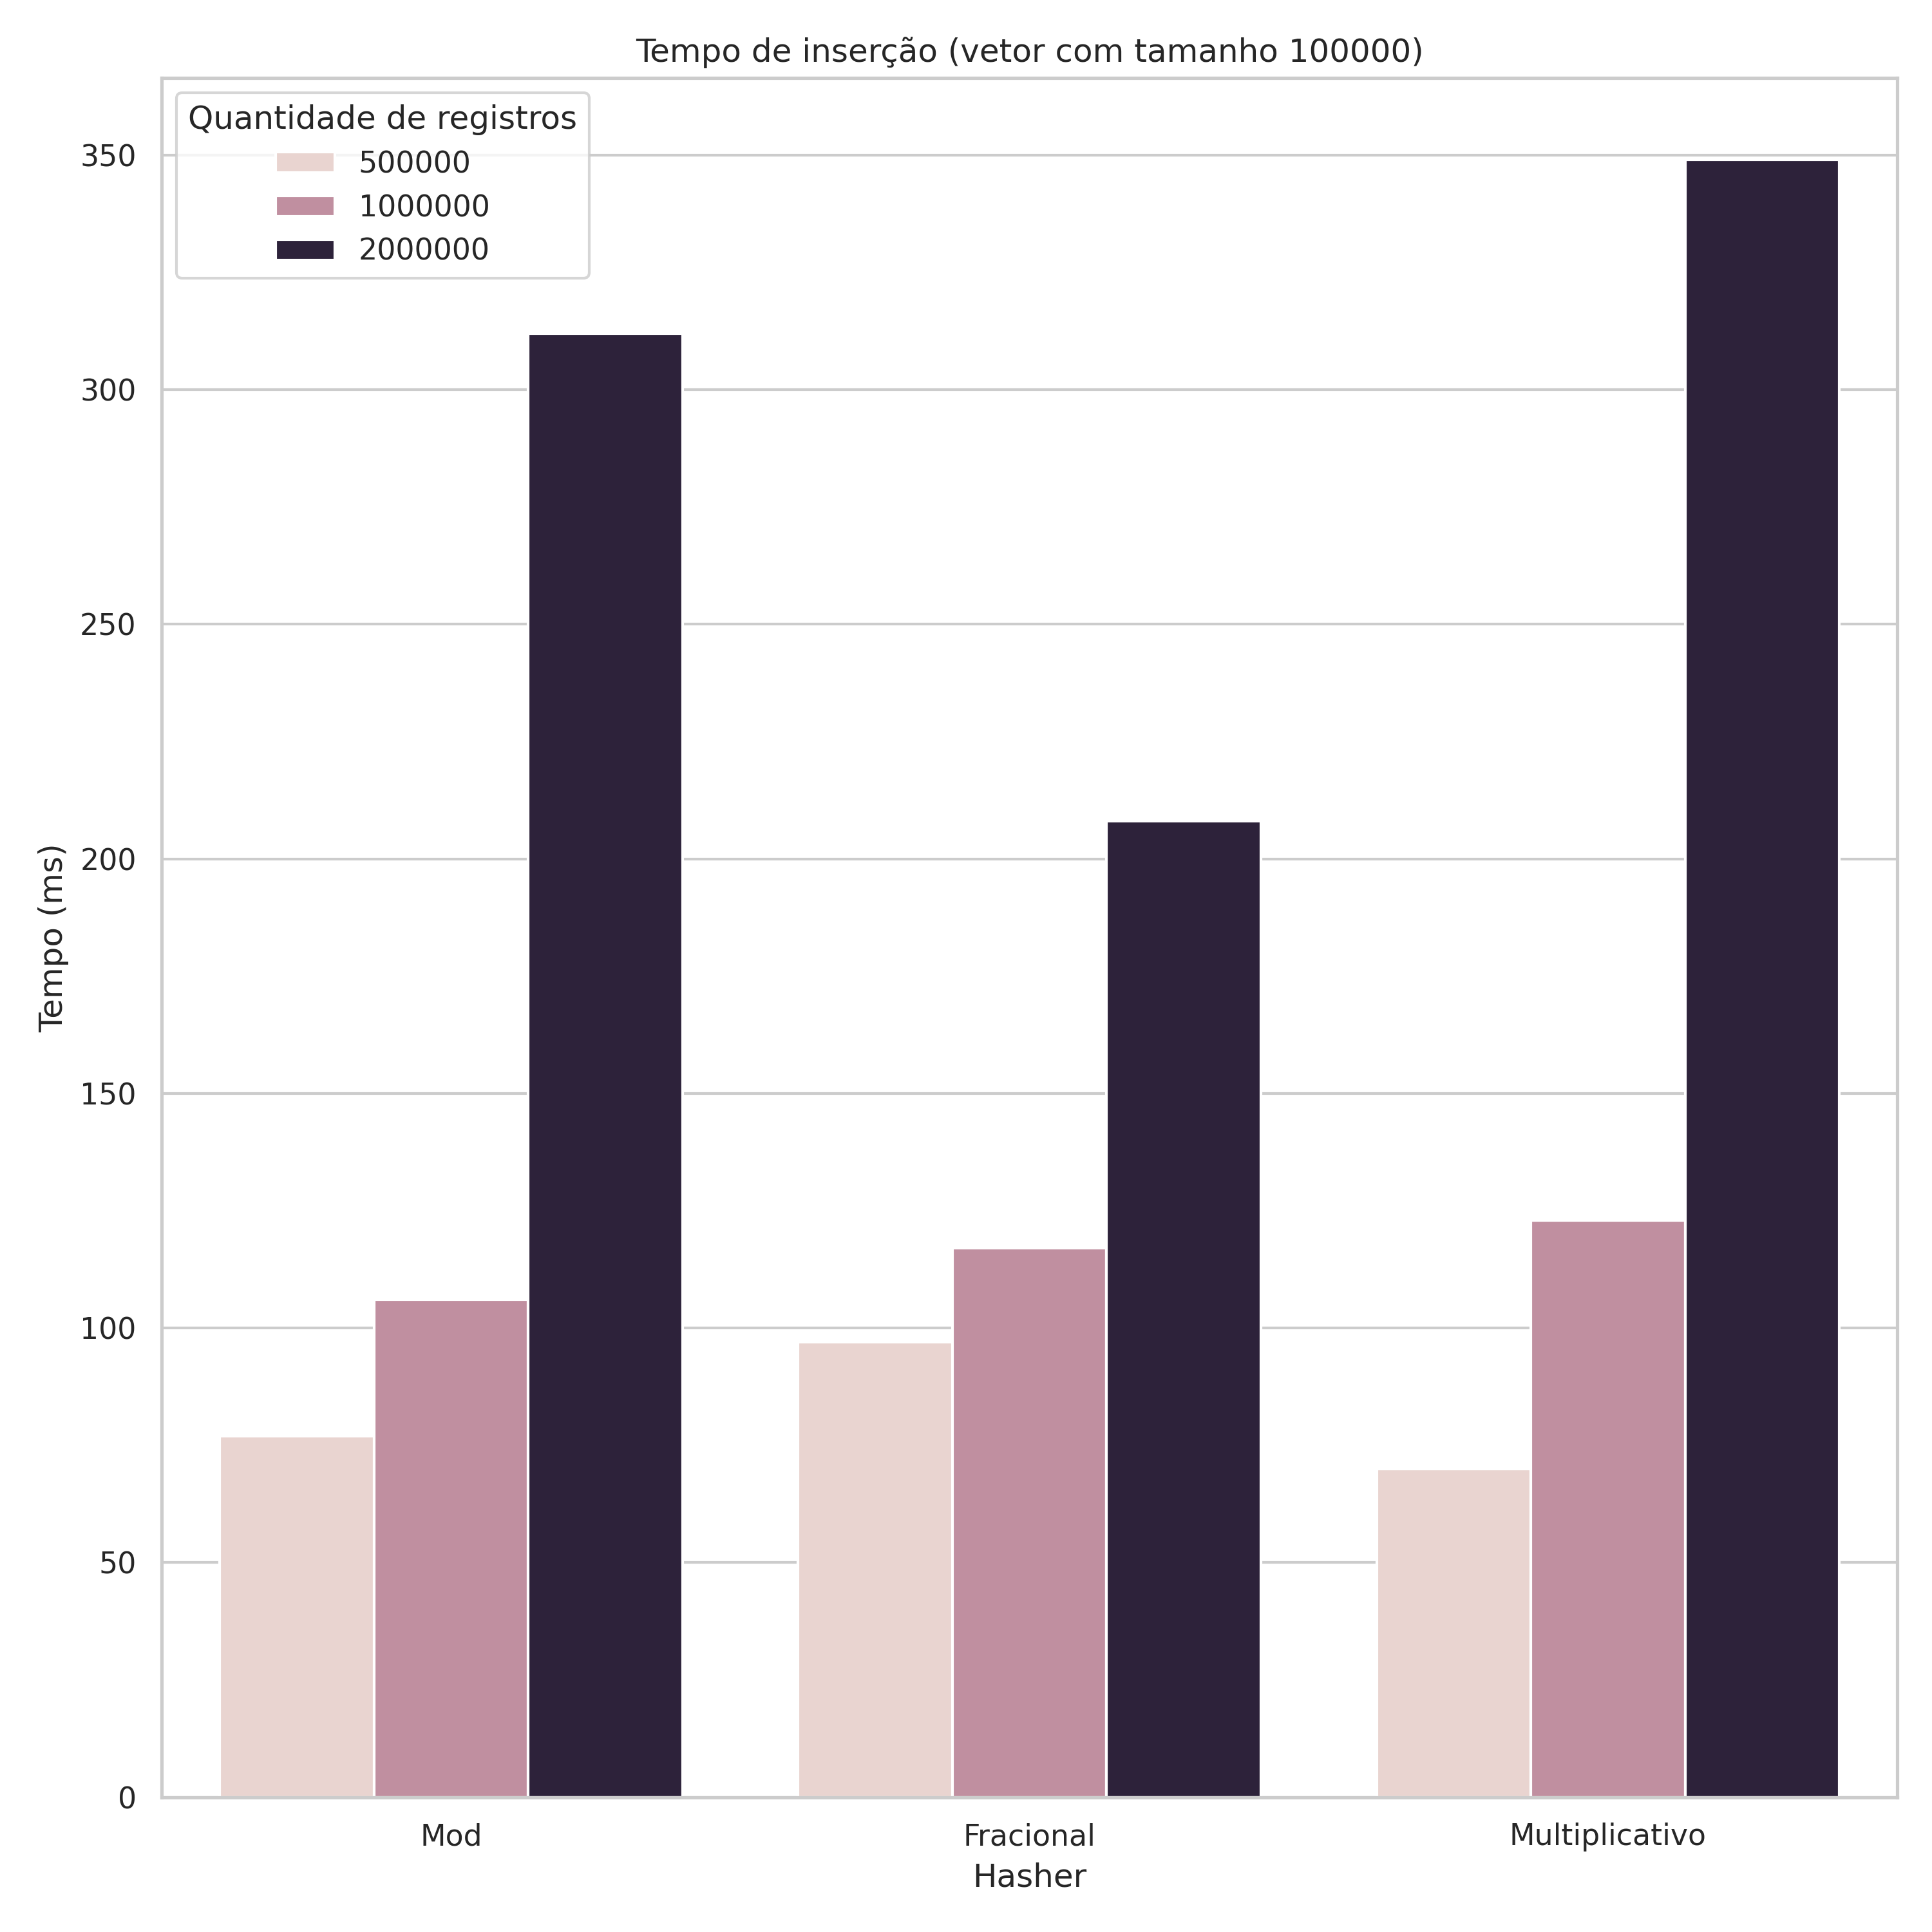
\includegraphics[width=\textwidth,height=\textheight,keepaspectratio]{figures/insertion_runtime_100000.png}
\caption{Tempo para inserir todos os registros gerados em cada uma das funções hash, com uma tabela com capacidade para 100,000 elementos.}
\end{figure}

\newpage
\begin{figure}[ht]
\centering
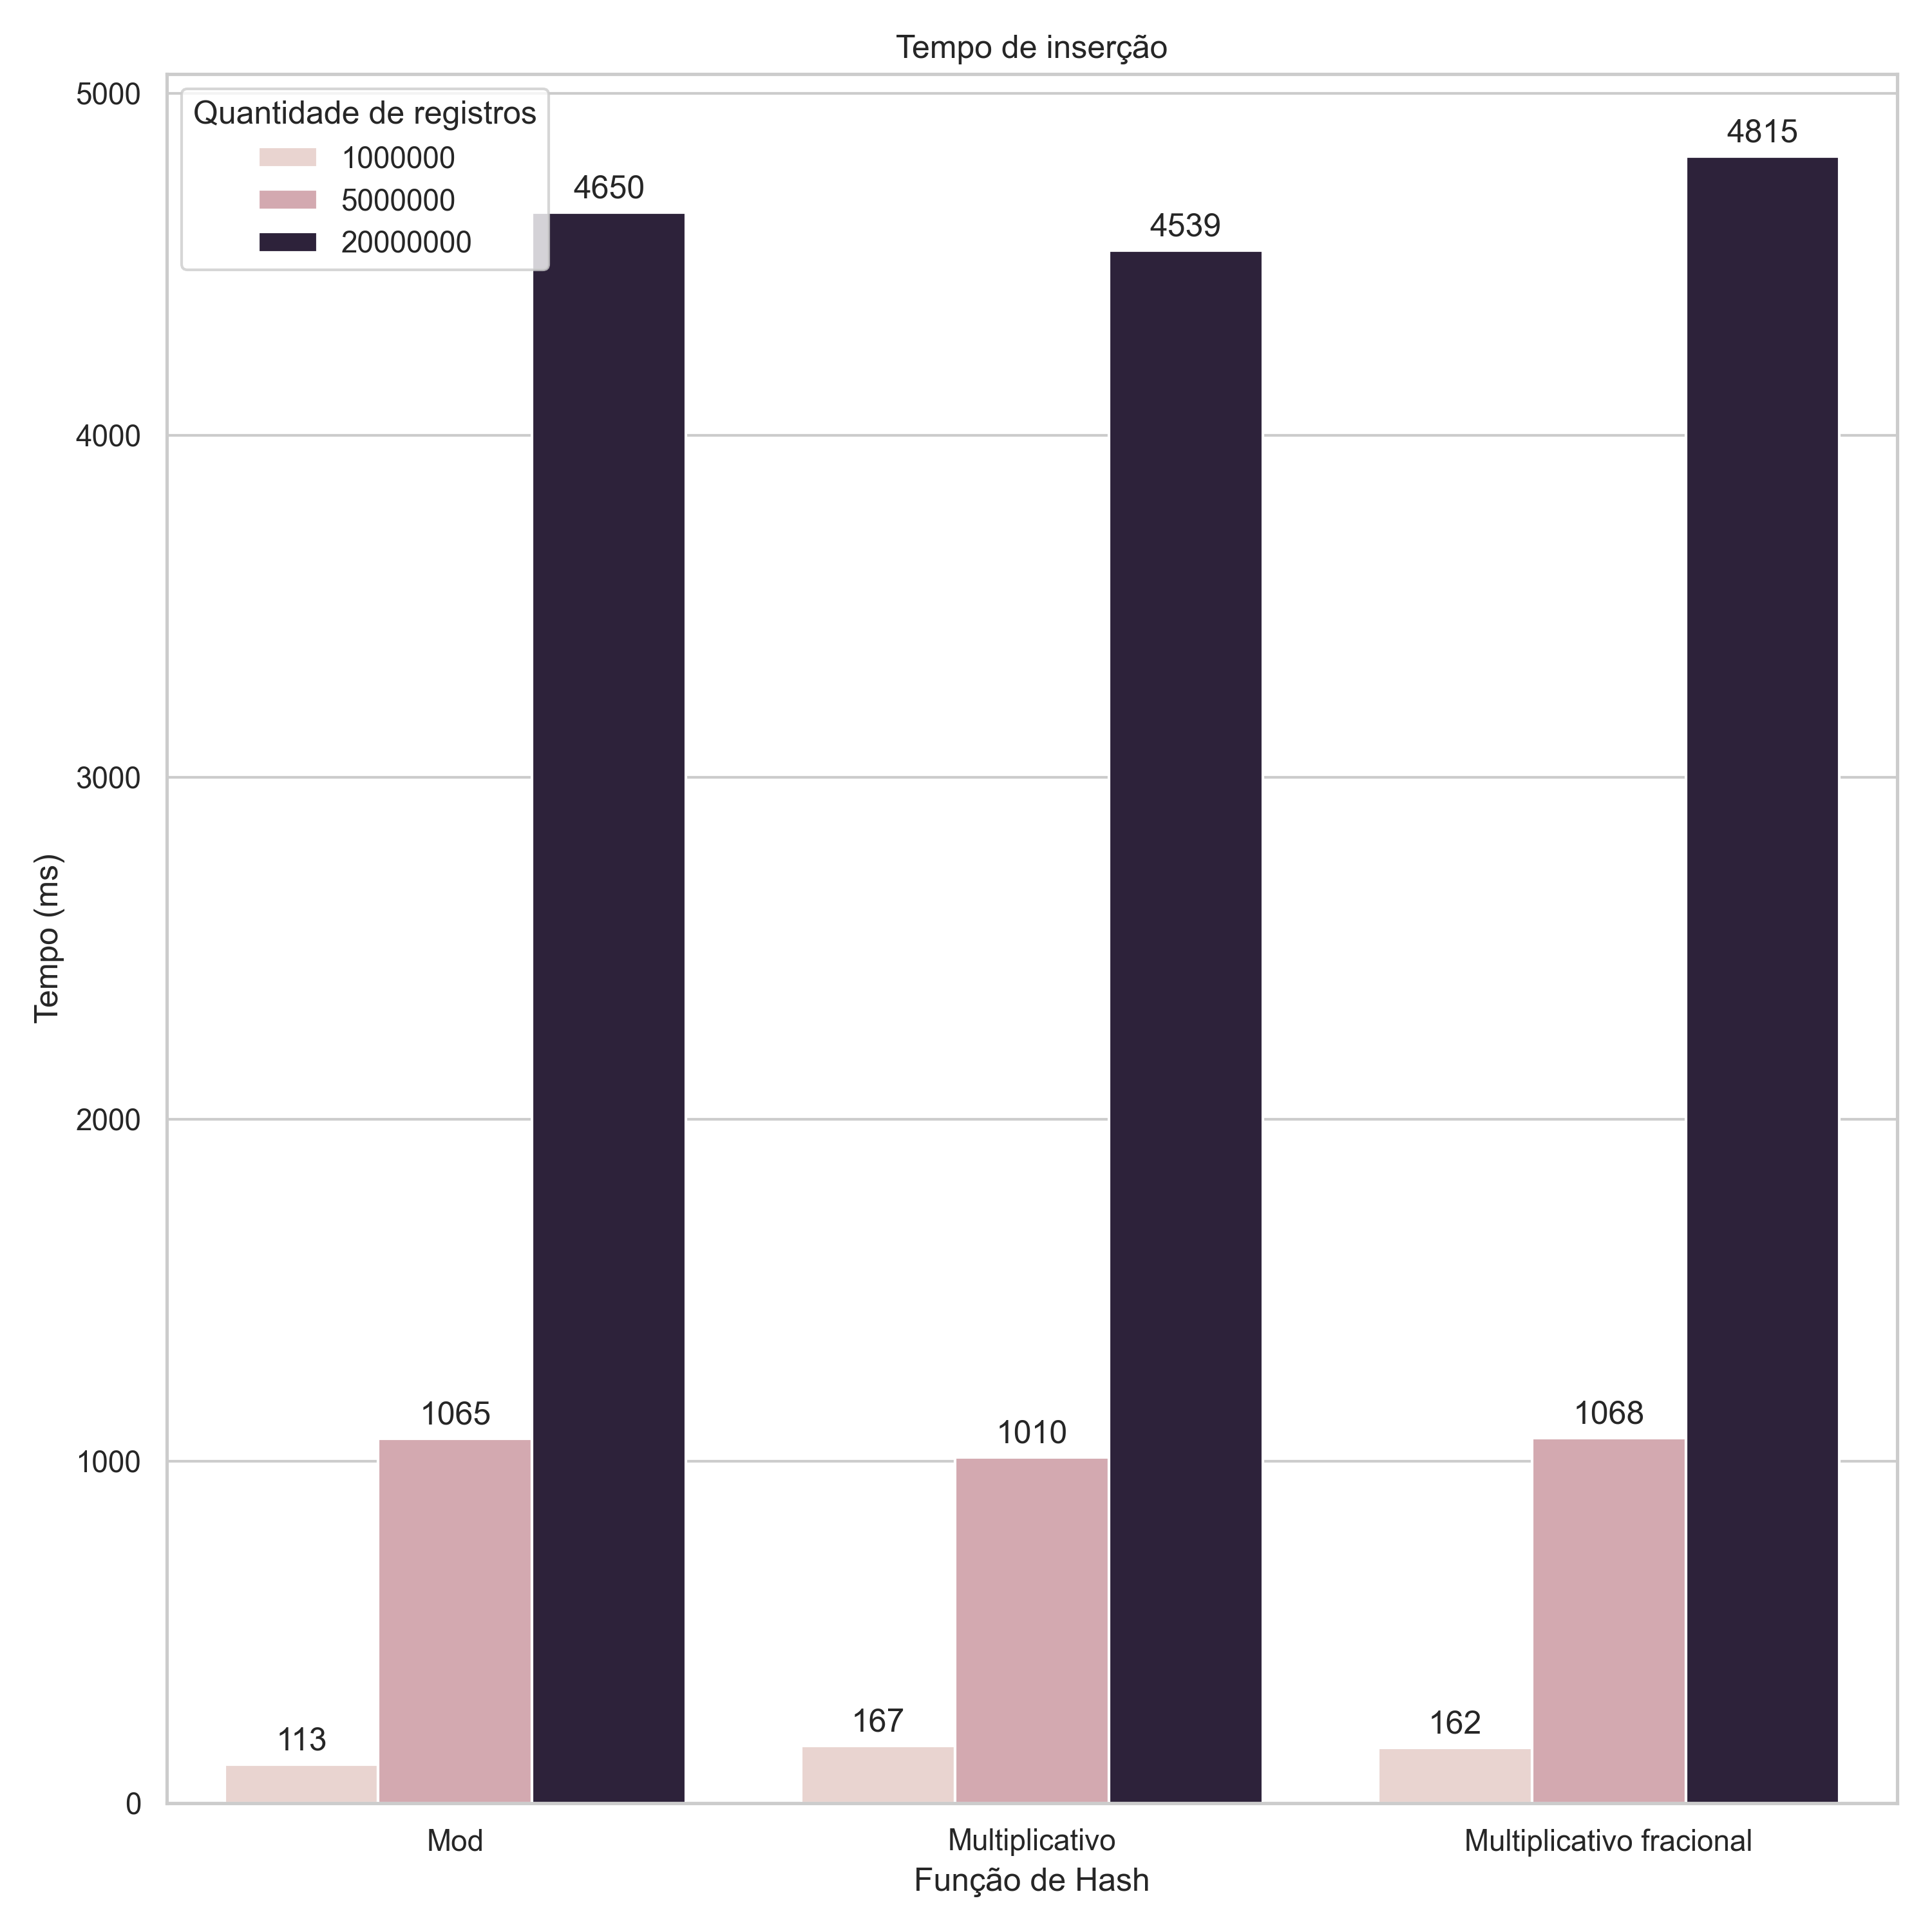
\includegraphics[width=\textwidth,height=\textheight,keepaspectratio]{figures/insertion_runtime_500000.png}
\caption{Tempo para inserir todos os registros gerados em cada uma das funções hash, com uma tabela com capacidade para 500,000 elementos.}
\end{figure}

\newpage
\begin{figure}[ht]
\centering
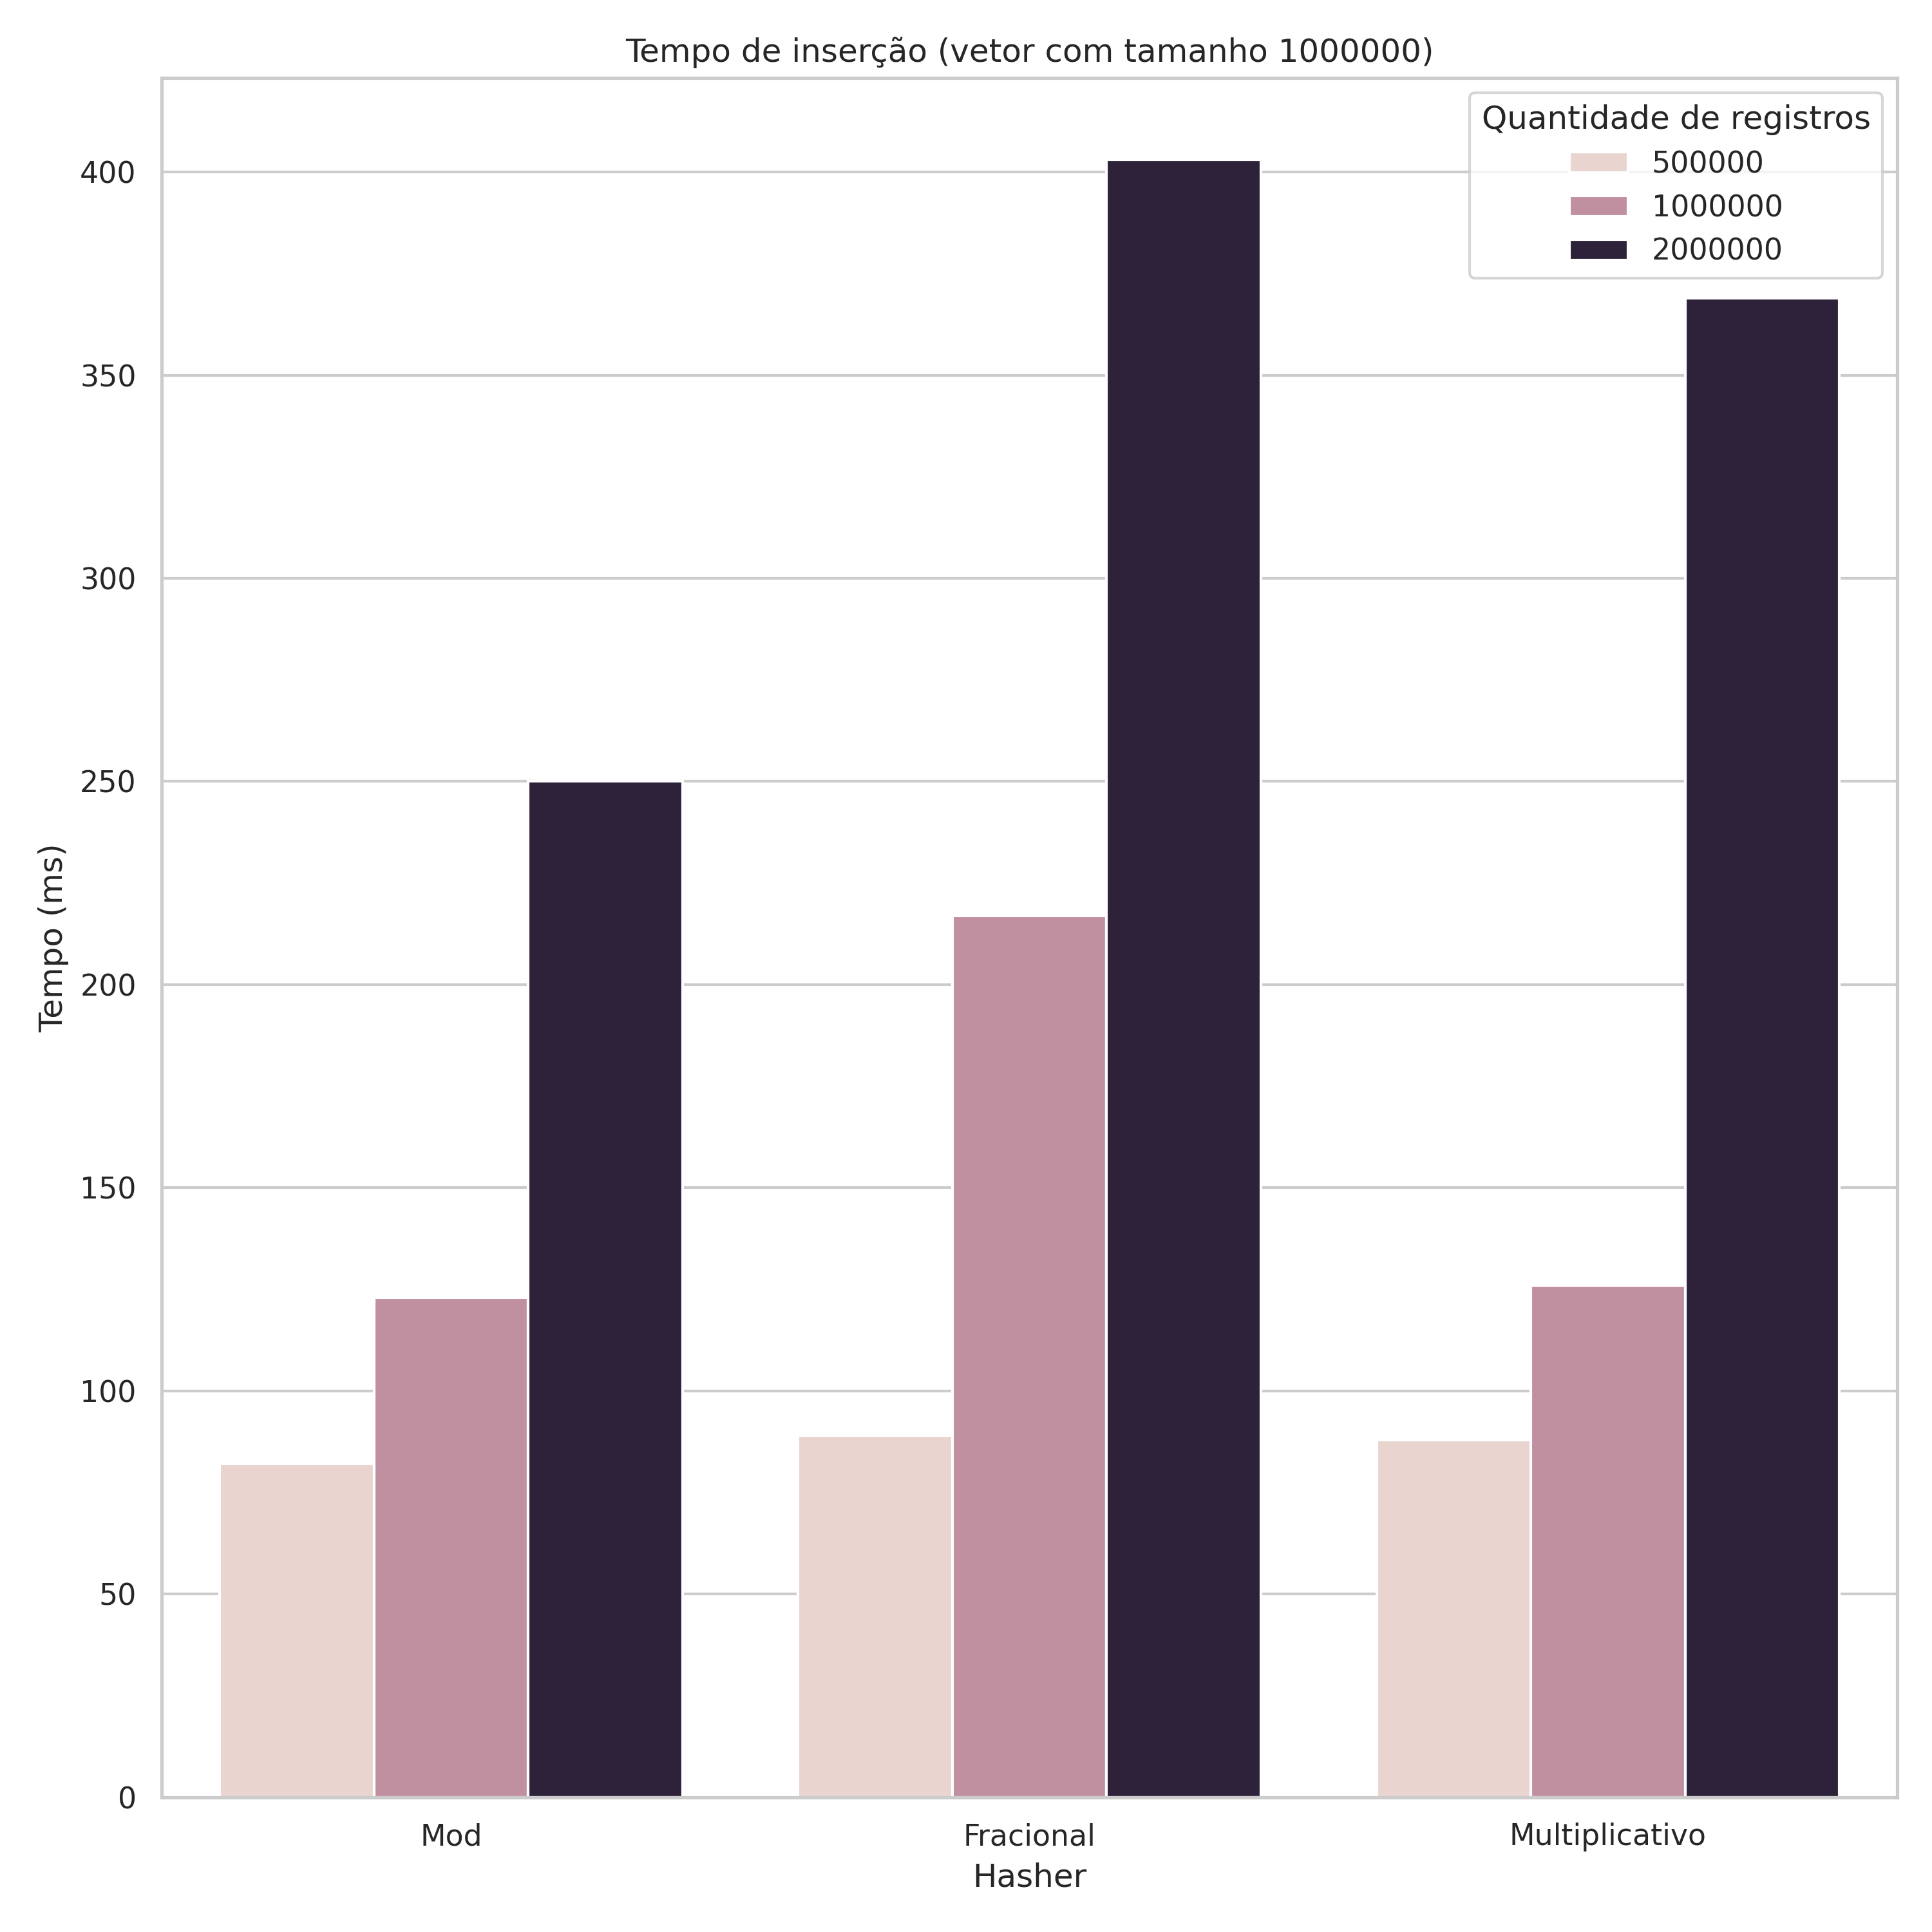
\includegraphics[width=\textwidth,height=\textheight,keepaspectratio]{figures/insertion_runtime_1000000.png}
\caption{Tempo para inserir todos os registros gerados em cada uma das funções hash, com uma tabela com capacidade para 1,000,000 elementos.}
\end{figure}

\newpage
\subsection{Análise}
Baseado nos resultados, concluímos que a função de hash sozinha não tem grandes impactos na performance de inserção. O principal fator de lentidão é a quantidade de registros em sí a serem inseridos.
Esse resultado se deve, principalmente, ao fato de executarmos somente operações de tempo constante na inserção: a hash da chave e a inserção na lista encadeada.

\newpage
\section{Busca de registros}

\subsection{Amostras}

\begin{figure}[ht]
\centering
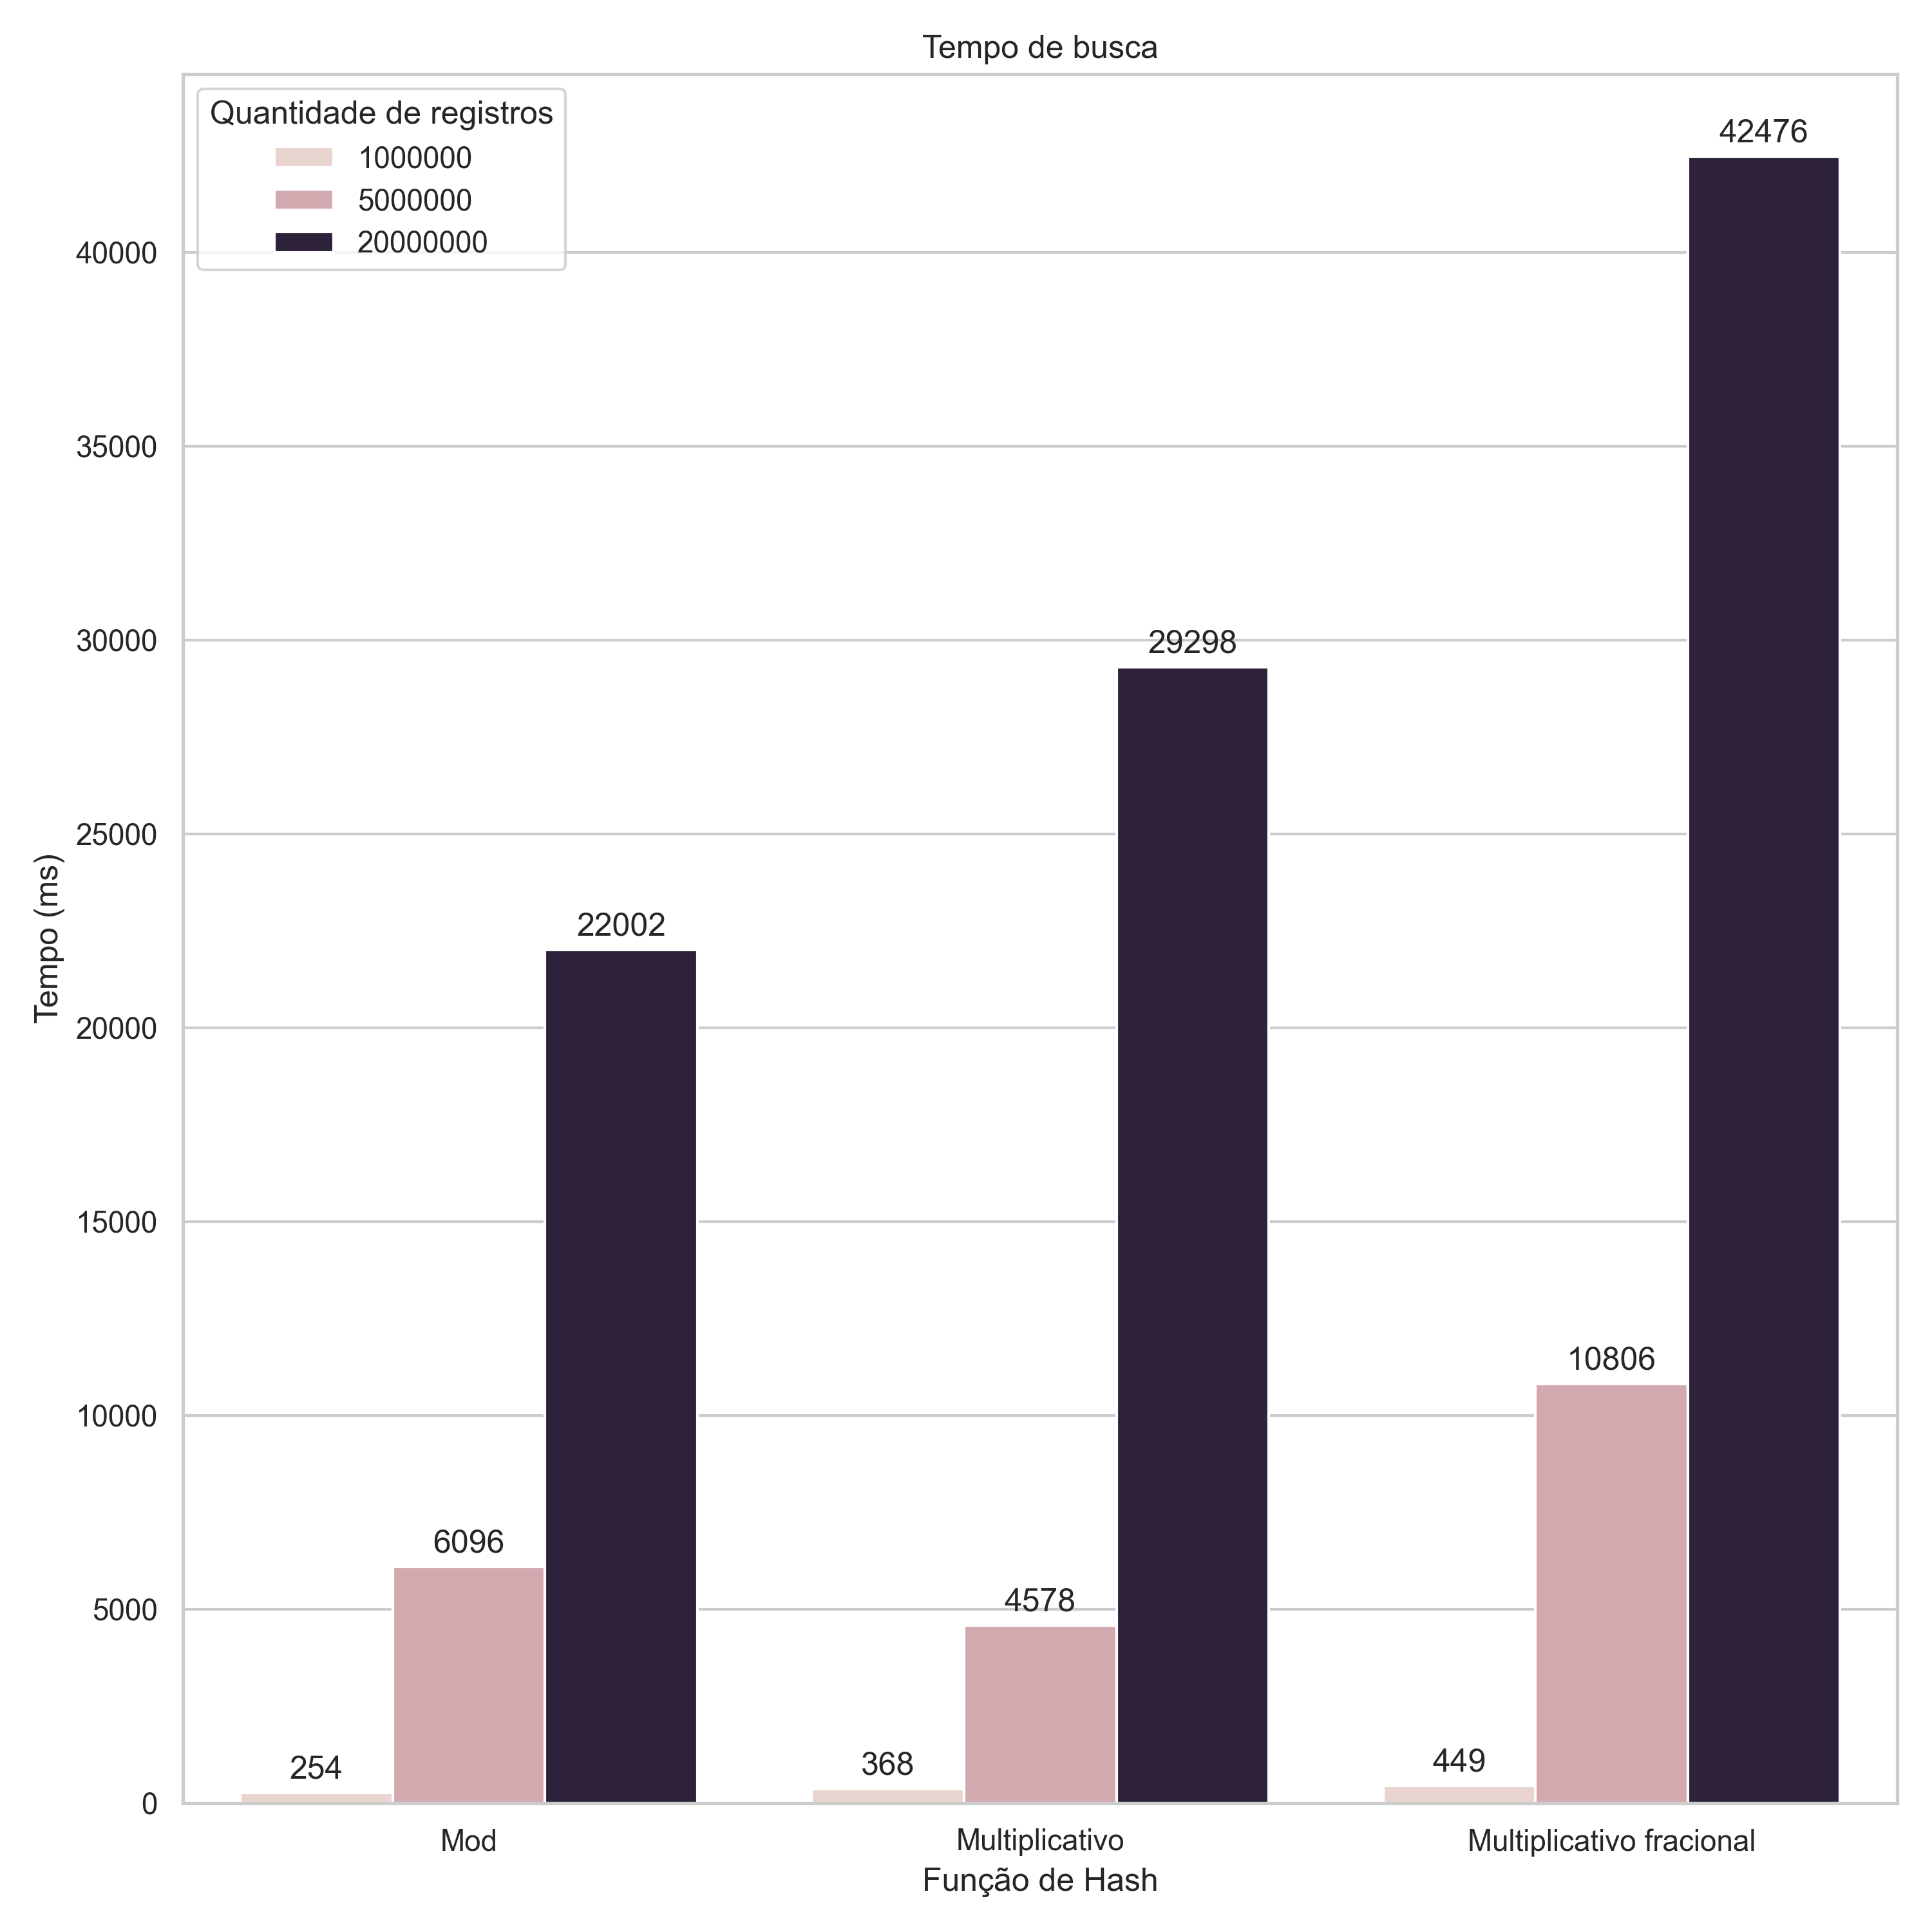
\includegraphics[width=\textwidth,height=\textheight,keepaspectratio]{figures/lookup_runtime_100000.png}
\caption{Tempo para buscar todos os registros gerados em cada uma das funções hash, com uma tabela com capacidade para 100,000 elementos.}
\end{figure}

\newpage
\begin{figure}[ht]
\centering
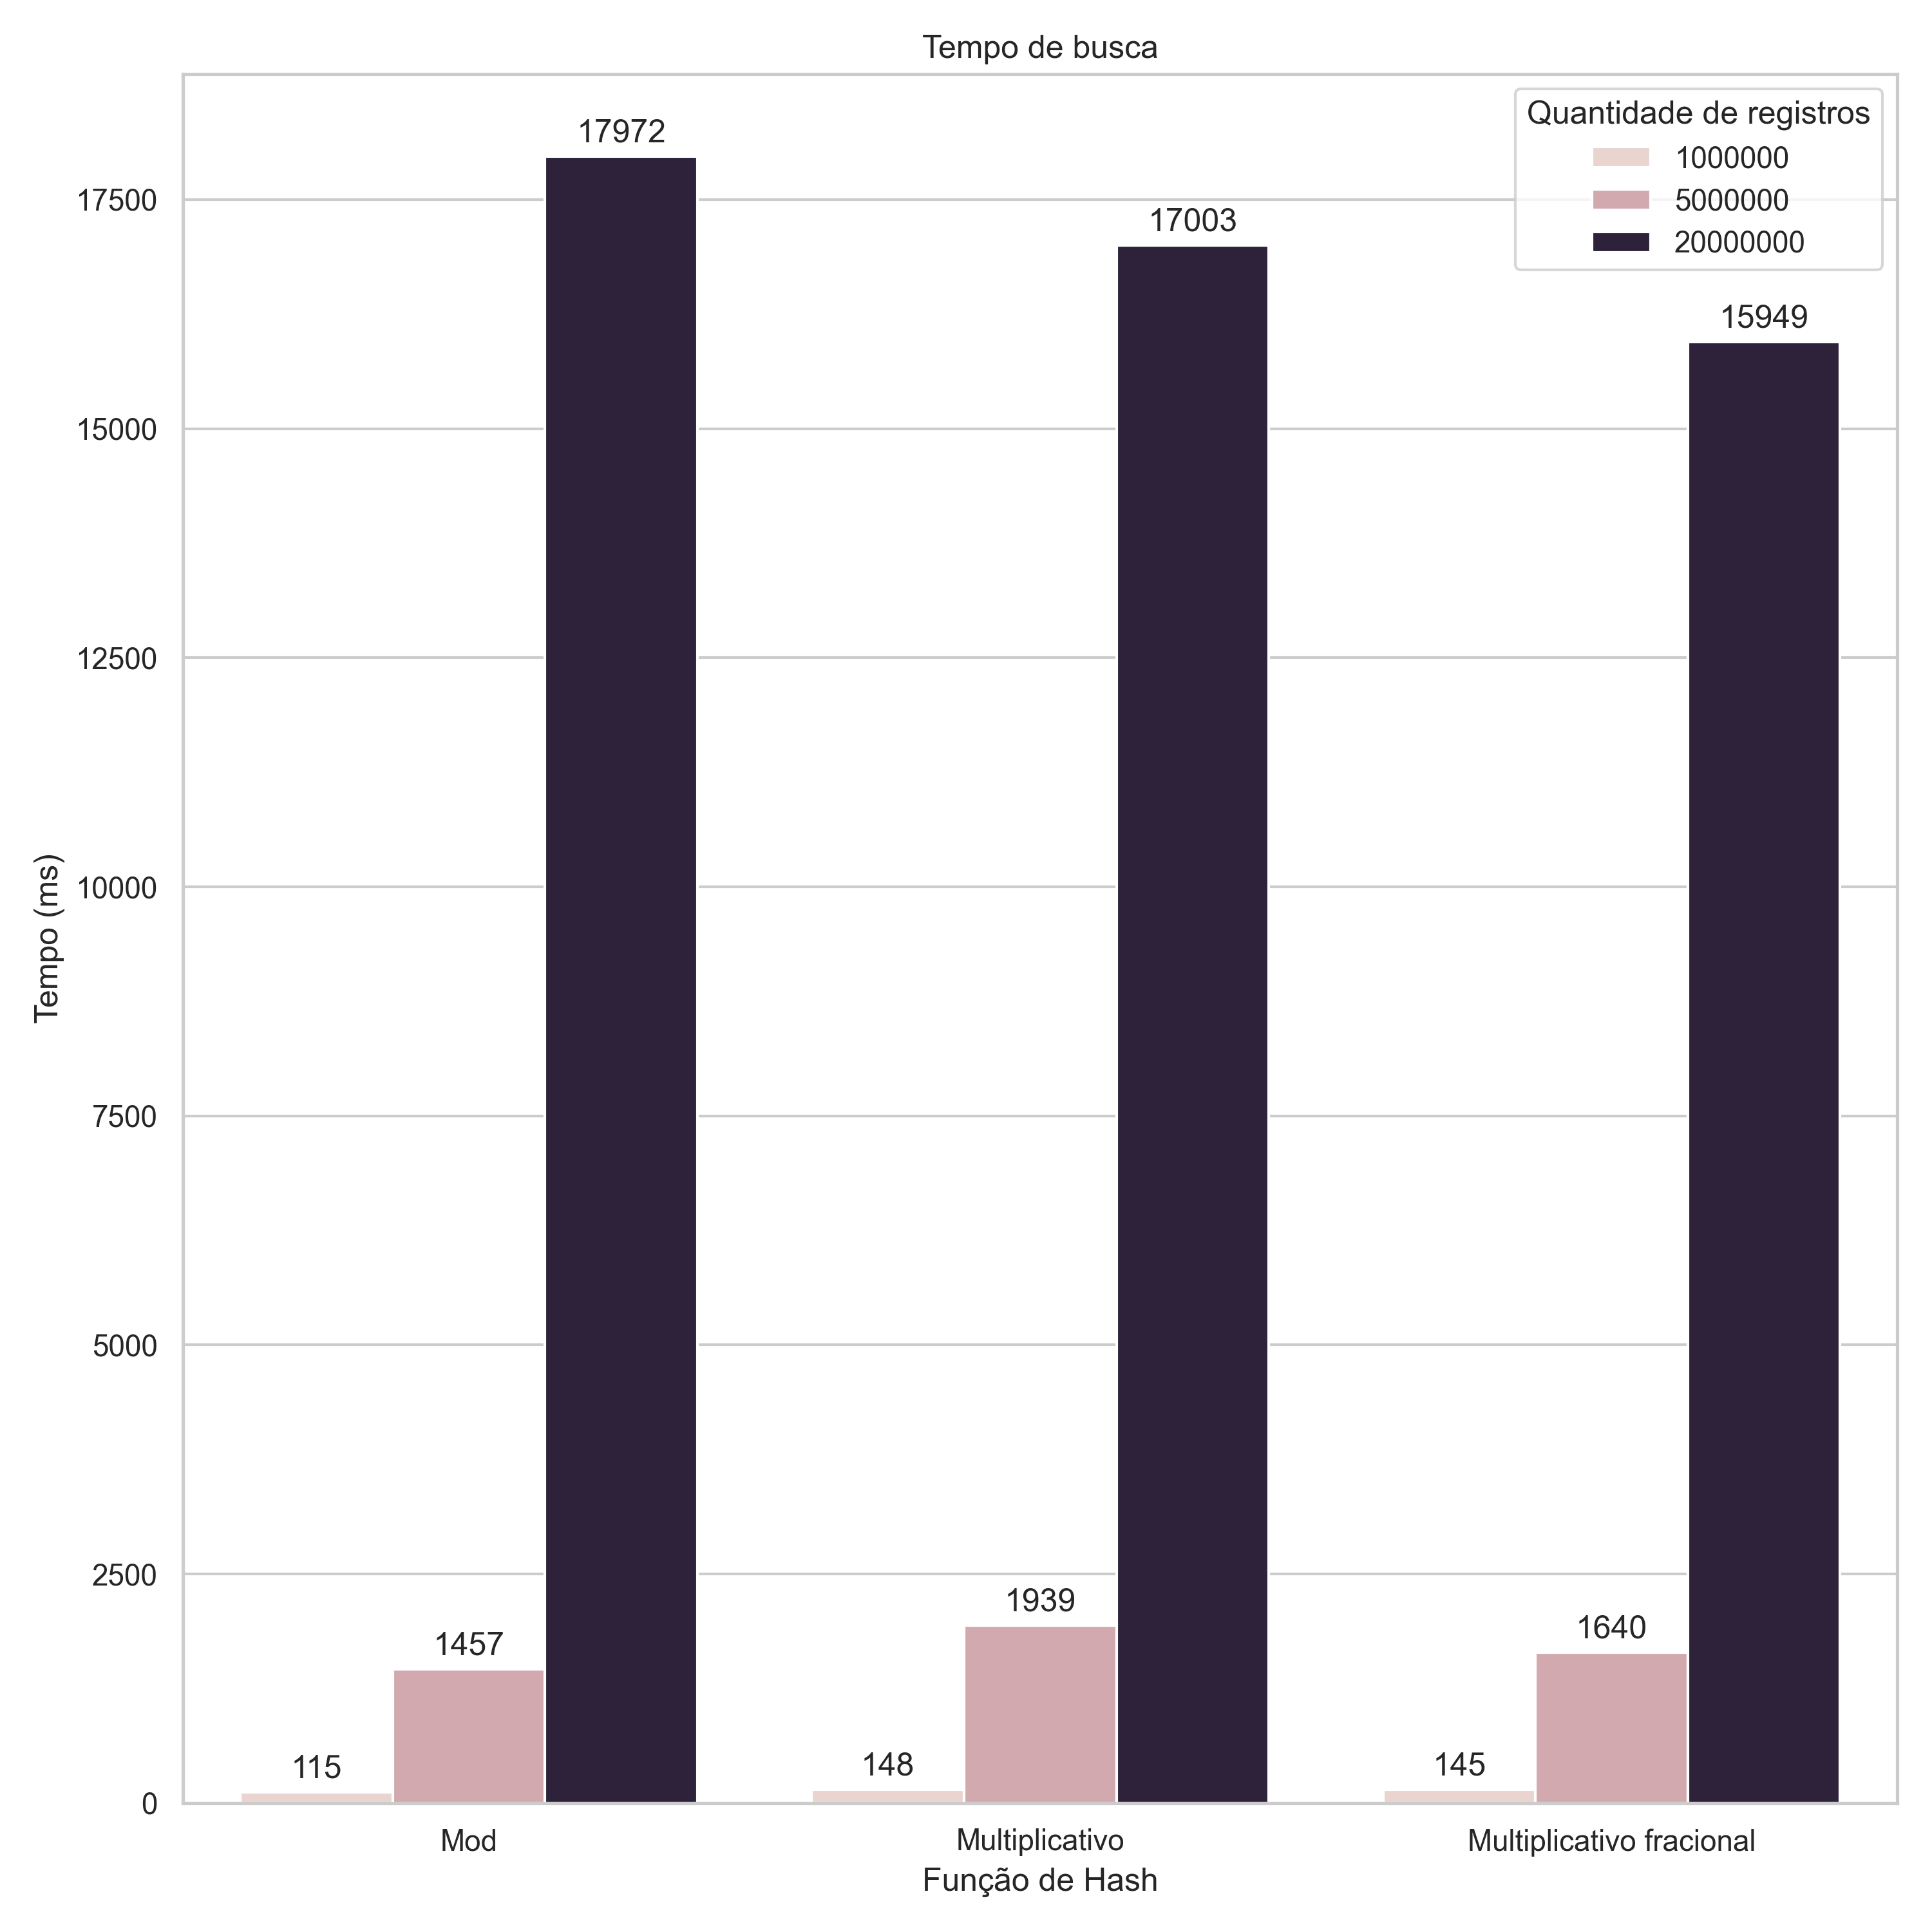
\includegraphics[width=\textwidth,height=\textheight,keepaspectratio]{figures/lookup_runtime_500000.png}
\caption{Tempo para buscar todos os registros gerados em cada uma das funções hash, com uma tabela com capacidade para 500,000 elementos.}
\end{figure}

\newpage
\begin{figure}[ht]
\centering
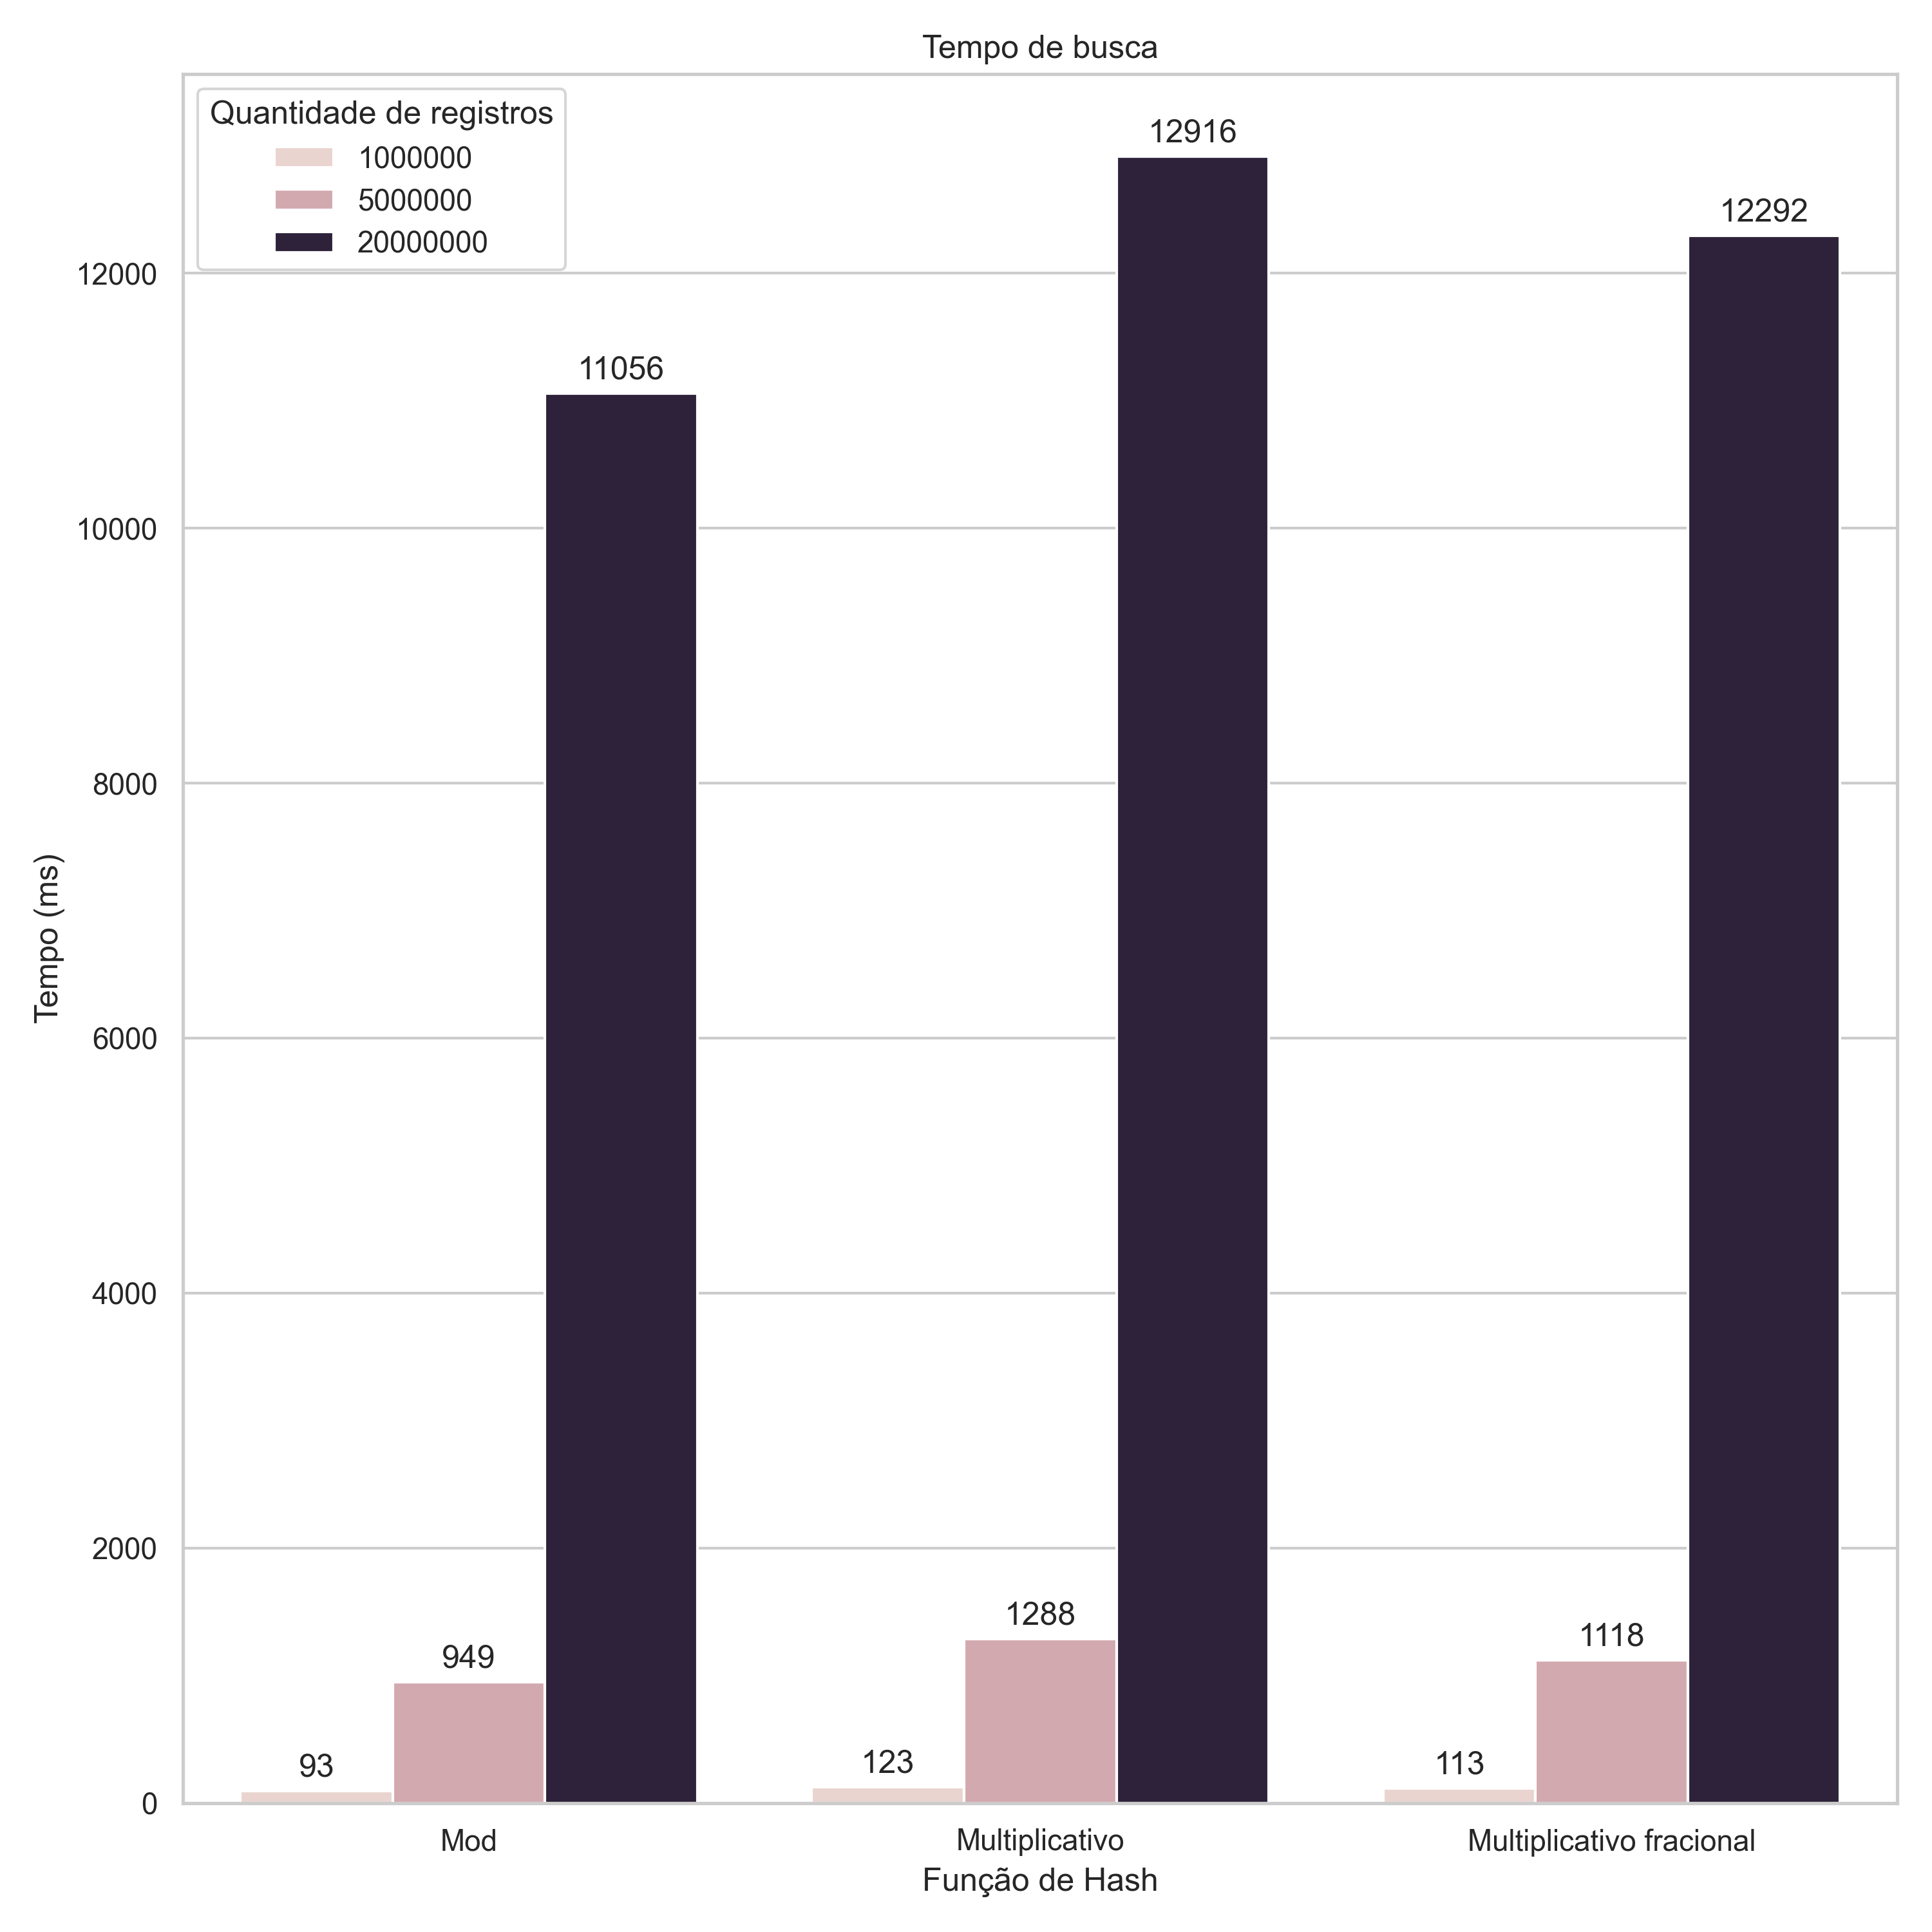
\includegraphics[width=\textwidth,height=\textheight,keepaspectratio]{figures/lookup_runtime_1000000.png}
\caption{Tempo para buscar todos os registros gerados em cada uma das funções hash, com uma tabela com capacidade para 1,000,000 elementos.}
\end{figure}

\newpage
\subsection{Análise}
A busca nos dá resultados mais interessantes, principalmente quando está sendo buscado uma grande quantidade de elementos, destacando as diferenças entre cada uma das funções hash.
As duas variações de hash multiplicativas tendem a ter pior performance comparada a hash de mod, que é mais simples. Isso pode indicar uma má escolha na constante usada para multiplicação,
que, na nossa implementação, foram duas constantes concebidas por Donald Knuth.


\end{document}
